\documentclass{article}

\usepackage{fancyhdr}
\usepackage{graphicx}

\usepackage{xepersian}
\settextfont{XB Zar}

\setlength{\parindent}{0pt}

\title{

\includegraphics[width=0.4\textwidth]{sharif.png}\\
\normalsize{دانشکده مهندسی کامپیوتر}\\
\vspace{1cm}
	
\huge{طراحی پایگاه‌داده}
\\ \vspace{.8cm}
\Large{داک نهایی پروژه}
}

\author{
\\
دکتر امینی
\\ \vspace{.4cm}
\\
  سارا آذرنوش       ---      98170668
\\ \vspace{0.2cm} \\
  سید ارشان دلیلی       ---      98105751
\\ \vspace{0.2cm} \\
  پارسا محمدیان       ---      98102284
\\ \vspace{.4cm}
}

\date{\today}

\begin{document}

\clearpage
\maketitle
\thispagestyle{empty}

\newpage

\clearpage
\pagestyle{fancy}
\lhead{طراحی پایگاه‌داده}

\rhead{داک نهایی پروژه}

\tableofcontents

\newpage

\setcounter{page}{1}


\section{فاز صفر}
 در فاز صفر پروژه ابتدا نوع موجودیت‌های شرکت کننده در یک بانک الکترونیکی و هم‌چنین نیازمندی‌های موجود در آن را به دست آوردیم و سپس ویژگی‌ها و صفات مورد نیاز این نوع موجودیت‌ها را مطابق با ذات مسئله به دست آوردیم.
(داک فاز صفر در فایل زیپ قرار دارد.)

\section{فاز اول}

در فاز ۱ پروژه، ابتدا اصلاحات لازم در نیازها را اعمال کردیم و سپس نمودار EER محیط را ترسیم کردیم و روابط موجود بین نوع موجودیت‌ها را مطابق آن مدل کردیم. در این فاز سعی شد روابط موجود بین نوع موجودیت‌ها تا حد خوبی رعایت شوند که بازتاب دنیای واقعی باشند.
(فایل مربوط به فاز ۱ در فایل زیپ قرار دارد.)
\section{فاز دوم}

در فاز دوم پروژه، جدول‌های مورد نیاز در پایگاه داده را مطابق نمودار EER فاز۱ و با توجه به درجه روابط بین موجودیت‌ها در نمودار EER .به دست آوردیم تا بتوانیم با ساخت این جدول‌ها، پایگاه داده را پیاده‌سازی کنیم.
(فایل مربوط به فاز ۲ در فایل زیپ قرار دارد.)


\section{فاز سوم}
\subsection{طراحی جداول به زبان \lr{SQL}}

در این بخش از این فاز، ابتدا به نرمالسازی جداول پرداختیم. جداول تا حد خوبی نرمال بودند و فقط تغییرات جزئی داشتند. 
نسخه جدید جداول در شکل 
\ref{fig:tables}
آمده است. 

(روابط در سطح BCNF نرمالیتی قرار دارند.)

\begin{figure}[!htbp]
    \centering
    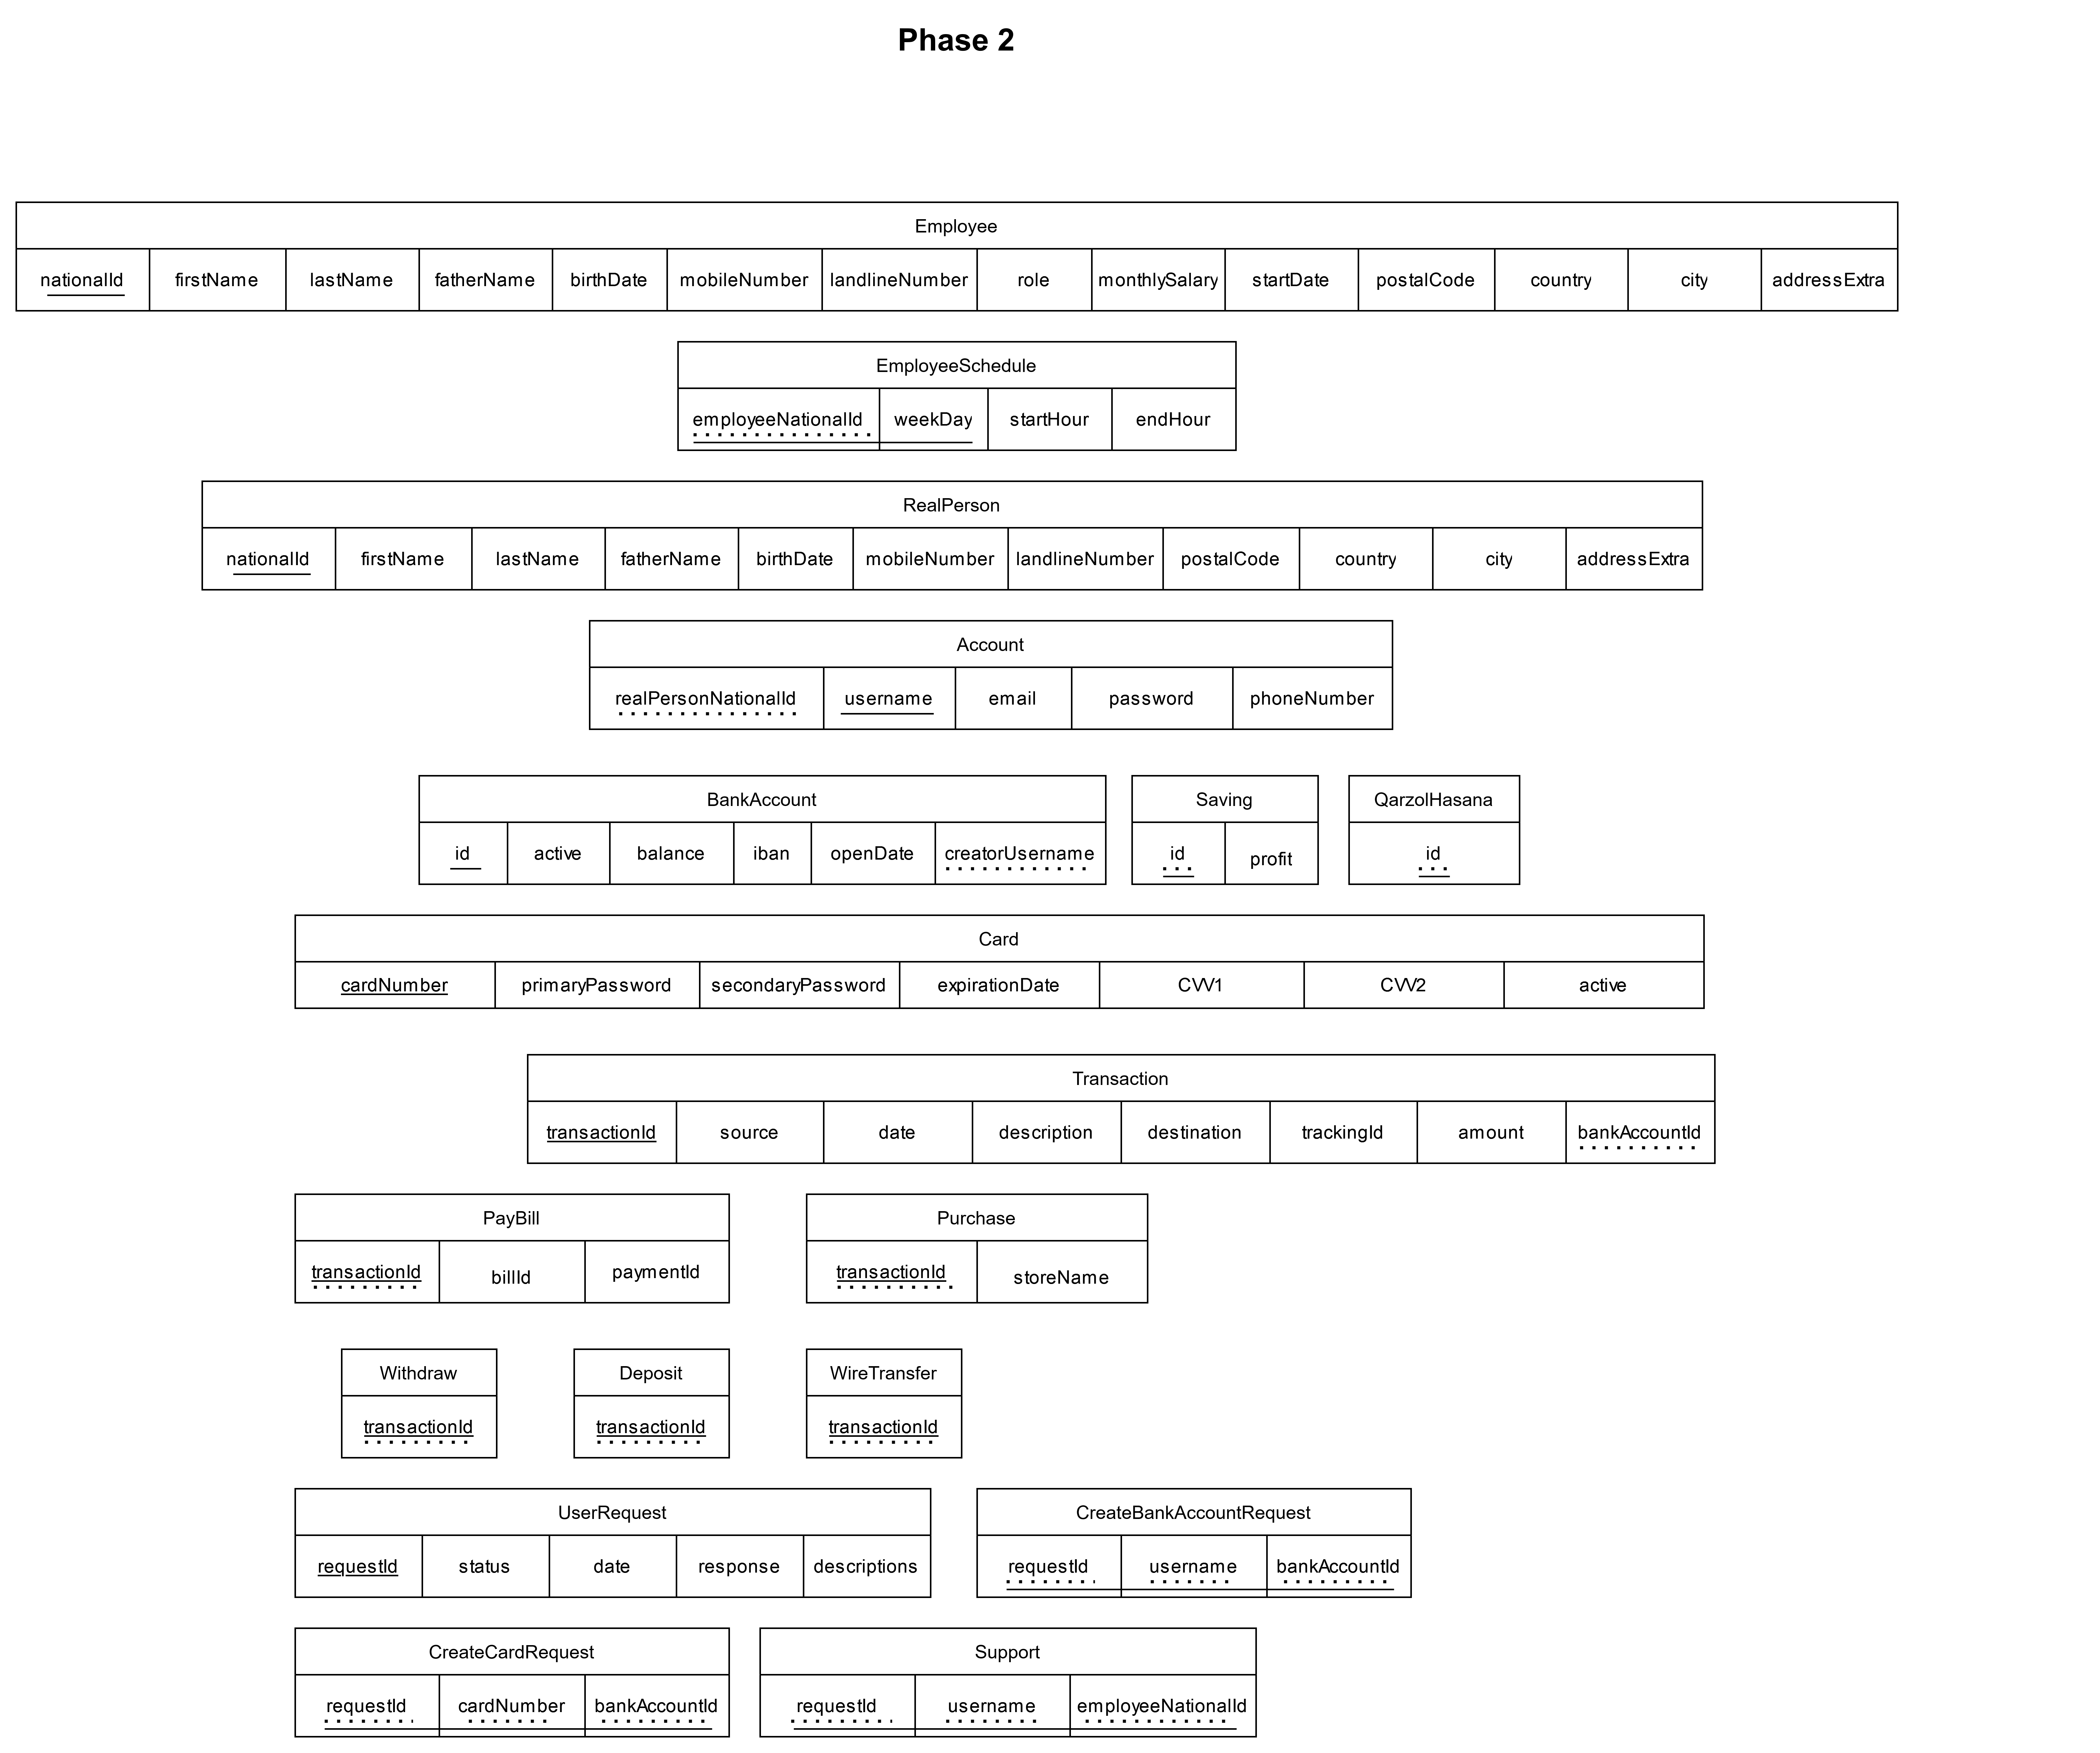
\includegraphics[width=0.8\textwidth]{../Phase 2 Modified.png}
    \caption{جداول نهایی}
    \label{fig:tables}
\end{figure}

سپس جداول مورد نیاز با زبان
\lr{SQL} 
پیاده‌سازی شدند. در پیاده‌سازی موارد زیر در نظر گرفته شدند. 

\begin{itemize}
    \item محدودیت‌های جامعیتی
    \item دیتاتایپ‌ها و دامنه صفات (این موارد، در فایل Data Types موجود می‌باشند.)
\end{itemize}


در ادامه با توجه به محدودیت‌های جامعیتی، به نوشتن رهانا میپردازیم. این کوئری‌ها در فایل 
\lr{database-query/tables.sql}
قرار دارند.

\subsection{رهانا}
رهاناها در فایل \lr{database-query/triggers.sql}
قرار دارند.


\subsection{طراحی و پیاده‌سازی برنامه کاربردی}
برای پیاده‌سازی برنامه کاربردی که به پایگاه داده متصل شود از زبان پایتون و فریمورک جنگو استفاده کردیم. 
با استفاده از این ابزارها یک وب اپلیکیشن نوشتیم که بتواند درخوات کاربر را به صورت پارامتری دریافت کرده 
و داده را متناظر با آن از دیتابیس 
\lr{(PostgreSQL)}
خوانده و نمایش بدهد. خواندن داده از دیتابیس به وسیله 
\lr{ORM} 
موجود در این فریمورک انجام می‌شود. از آنجایی که کوئری به صورت پارامتریک فرستاده می‌شود، 
از حمله 
\lr{SQL Injection}
جلوگیری می‌شود. یعنی در صورتی که کاربری از کوئری 
\lr{SQL} 
داخل سرچ باکس استفاده نماید، ورودی او به دیتابیس ارسال نمی‌شود. جزئیات پیاده‌سازی این برنامه کاربردی در 
پوشه 
\lr{application} 
قابل مشاهده است. 

\end{document}